\section{Managing different configurations}

\subsection{Objectives}

	\begin{frame}
		\frametitle{Objective}
		
		Now that we have a worker in kubernetes, we wants to be able to configure it.
		
		Also, we want to be able to differenciate between development and production configuration.
		
	\end{frame}
	
\subsection{Use kustomize}	
	
	\begin{frame}
		\frametitle{Kustomize among other solutions}
		
		\begin{center}
		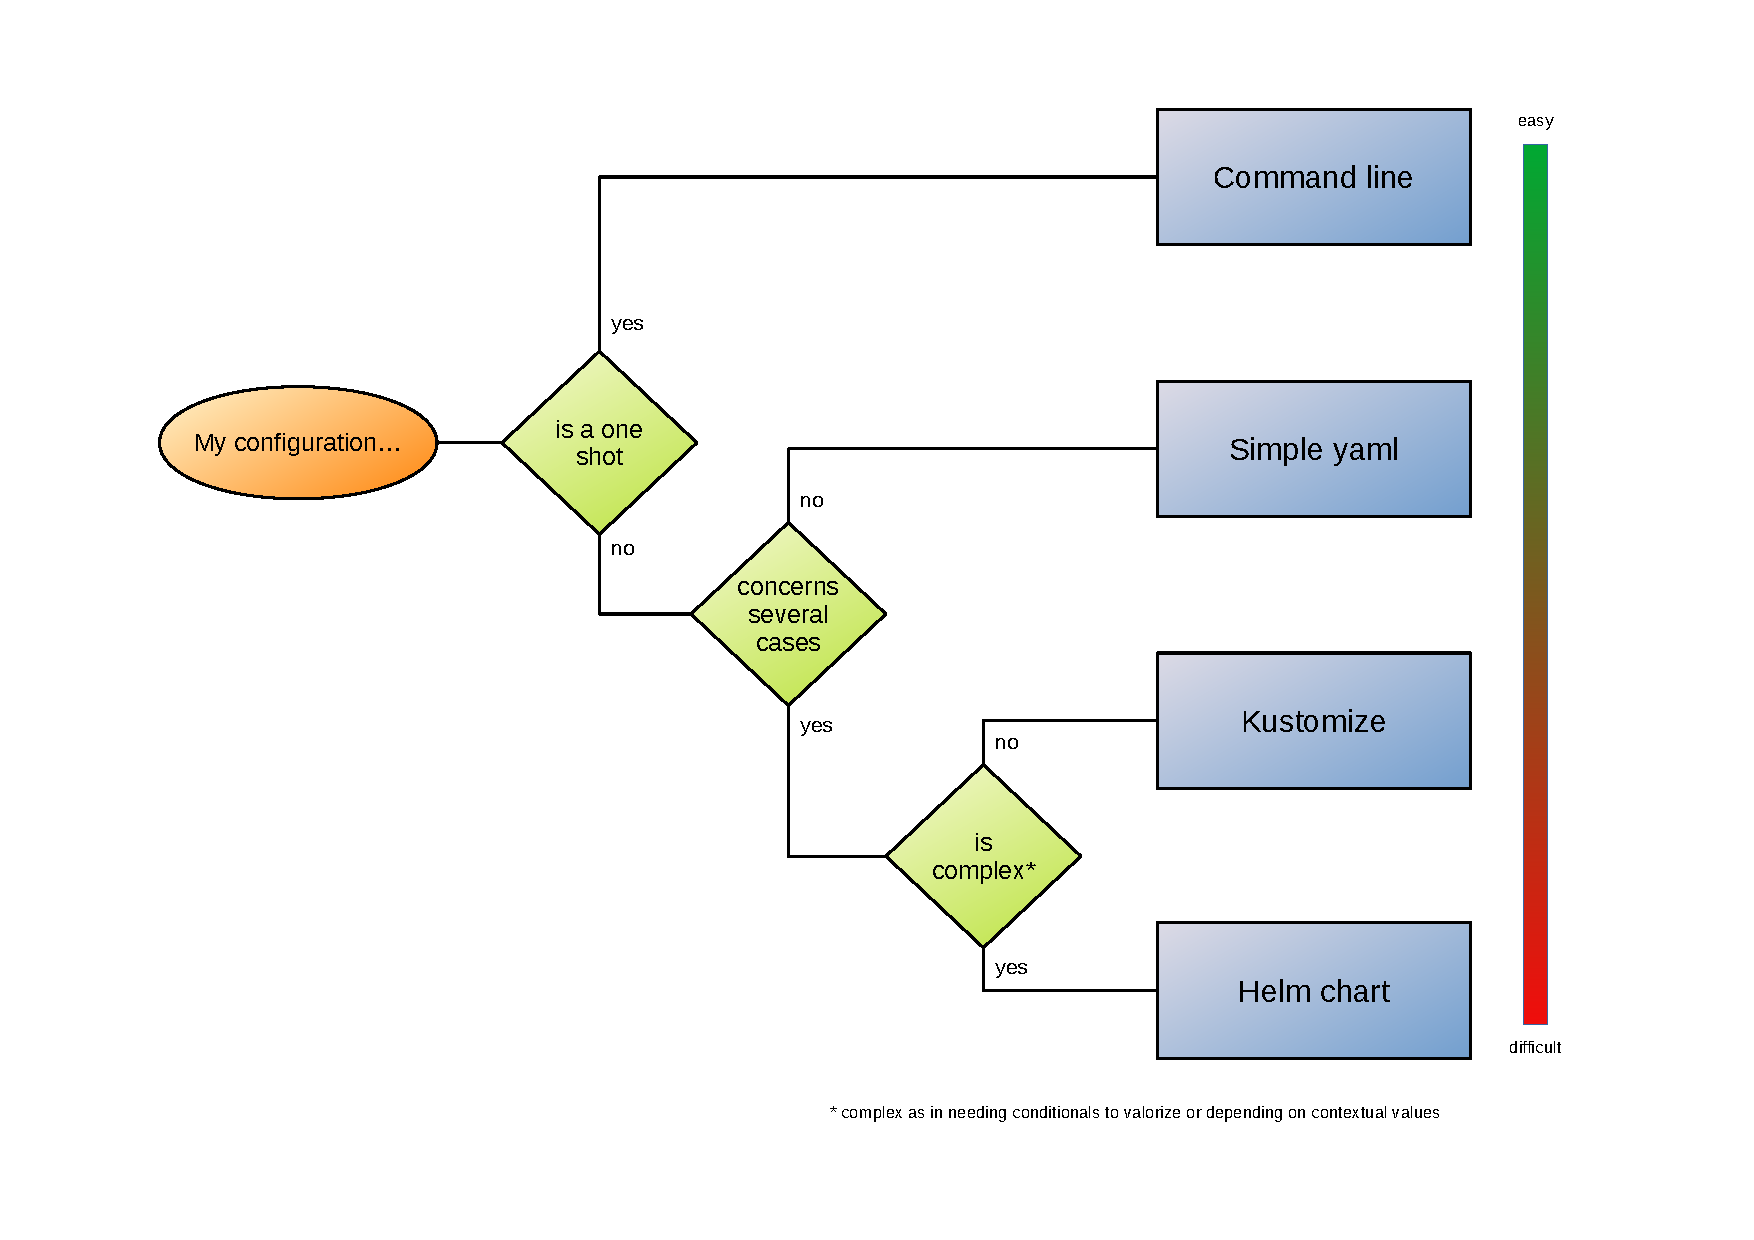
\includegraphics[height=7.5cm]{../../../resources/color/choiceConfigKind.pdf}
		\end{center}
	\end{frame}
	
	\begin{frame}
		\frametitle{Layer based configuration}
		
		Kustomize is a tool now integrated in kubectl.
		
		\bigskip
		It manage the configuration using a layer based system.
		
		That means that a configuration is the result of a base configuration, on wich layers are applyed.
		
		Eache layer can contains new resources or new patches.
		
		\bigskip
		As a base layer is considered as a resource, that enable to define a configuration as the concatenation of several other configurations and their patches.
	\end{frame}
	
	\begin{frame}[fragile]
		\frametitle{Initialize the base}
		
		We are creating a folder tree to sort our files
		\begin{block}{Command line 1}
			\begin{verbatim}
				mkdir kube
				cd kube
				mkdir base
				cd base
			\end{verbatim}
		\end{block}
	\end{frame}
	
	\begin{frame}[fragile]
		\frametitle{Initialize the base}
		
		We are starting with a fresh new deployment.yaml
		\begin{block}{source.yaml}
			\begin{tiny}
				\begin{verbatim}
						apiVersion: apps/v1
					kind: Deployment
					metadata:
					  name: worker
					  labels:
					    tinkou: worker
					spec:
					  selector:
					    matchLabels:
					      tinkou: worker
					  template:
					    metadata:
					      labels:
					        tinkou: worker
					    spec:
					      containers:
					      - name: worker
					        image: <registry>/training/worker-<id>:v1
					      imagePullSecrets:
					      - name: regcred
				\end{verbatim}
			\end{tiny}
		\end{block}
	\end{frame}
	
	\begin{frame}[fragile]
		\frametitle{Initialize the base}
		\begin{block}{Command line 1}
			\begin{verbatim}
				touch kustomization.yaml
				kustomize edit fix
				kustomize edit add resource source.yaml
				kustomize build
				kubectl apply -k .
			\end{verbatim}
		\end{block}
	\end{frame}
	
	\begin{frame}[fragile]
		\frametitle{Initialize the base}
		As we modify an immutable field, we need to delete the previous deployment before:
		\begin{block}{Command line 1}
			\begin{verbatim}
				kubectl delete deployment worker
				kubectl apply -k .
			\end{verbatim}
		\end{block}
	\end{frame}
	
	\begin{frame}[fragile]
		\frametitle{Add a parameter to our worker}
		
		Modify the worker to use a parameter:
		\begin{block}{worker.sh}
			\begin{verbatim}
				while true; do
				  echo "I'm $NAME and it is $(date)"
				  sleep 2
				done
			\end{verbatim}
		\end{block}
	\end{frame}
	
	\begin{frame}[fragile]
		\frametitle{Deploy the new version in our cluster}
		
		First we need to create a new version of the image:
		\begin{block}{Command line 1}
			\begin{verbatim}
				docker build -t <registry>/training/worker-<id>:v2 \
				                ../../
				docker push <registry>/training/worker-<id>:v2
			\end{verbatim}
		\end{block}
	\end{frame}
	
	\begin{frame}[fragile]
		\frametitle{Deploy the new version in our cluster}
		
		Change the deployment configuration:
		\begin{block}{source.yaml}
			\begin{small}
				Replace v1 by v2
			
				Add to the containers spec part:
				\begin{verbatim}
					spec:
					  containers:
					    env:
					    - name: NAME
					      value: <myName>
				\end{verbatim}
			\end{small}
		\end{block}
		
		And finaly apply the modification:
		\begin{block}{Command line 1}
			\begin{small}
					\begin{verbatim}
					kubectl apply -k .
				\end{verbatim}
			\end{small}
		\end{block}
	\end{frame}
	
	\begin{frame}
		\frametitle{Deploy the new version in our cluster}
		
		There are too many operations.
		
		\bigskip
		Is there a way to simplify this?
	\end{frame}
	
\subsection{Use skaffold}	
	
	\begin{frame}
		\frametitle{Skaffold}
		
		Skaffold is a developper oriented tool create to simplify the packaging and deployment on kubernetes.
		
		\medskip
		The Skaffold documentation can be found \href{https://github.com/GoogleContainerTools/skaffold}{her}.
		
		\medskip
		Installation documentation can be found \href{https://skaffold.dev/docs/getting-started}{here}.
	\end{frame}
	
	\begin{frame}[fragile]
		\frametitle{Initialize skaffold}
		
		Let's return in WORKER\_DIR and initialize skaffold:
		\begin{block}{Command line 1}
			\begin{verbatim}
				skaffold init
			\end{verbatim}
			Follow the application command line interface.
		\end{block}
	\end{frame}
	
	\begin{frame}[fragile]
		\frametitle{Initialize skaffold}

		By default skaffold detect the yaml, so it need to be configured to use kustomize:
		\begin{block}{skaffold.yaml}
			Remove the tag from the image
			
			\medskip
			Replace the block .deploy.kubectl by:
			\begin{verbatim}
				deploy:
				  kustomize:
				    path: kube/base			
			\end{verbatim}						
		\end{block}
	\end{frame}
	
	\begin{frame}[fragile]
		\frametitle{Using skaffold}
		
		We are going to test a little skaffold commands:
		\begin{block}{Command line 1}
			\begin{verbatim}
				skaffold build
				skaffold run
				skaffold delete
				skaffold dev
			\end{verbatim}					
		\end{block}
		
		Try to modify the file worker.sh.
	
	\end{frame}
	
	\begin{frame}[fragile]
		\frametitle{Create a kustomize layer for skaffold}
		
		Skaffold do not upgrade the image…
		\begin{block}{Command line 4}
			\begin{verbatim}
				kubectl describe deployment worker
			\end{verbatim}
		\end{block}
		
	\end{frame}
	
	\begin{frame}[fragile]
		\frametitle{Create a kustomize layer for skaffold}
		We need to let skaffold manage the image tag version, by created a dedicated configuration:
		\begin{block}{Command line 4}
			\begin{small}
				\begin{verbatim}
					cd kube
					mkdir skaffold
					vi patch.yaml
				\end{verbatim}
			\end{small}
		\end{block}
		
		\begin{block}{patch.yaml}
			\begin{tiny}
				\begin{verbatim}
					apiVersion: apps/v1
					kind: Deployment
					metadata:
					  name: worker
					spec:
					  template:
					    spec:
					      containers:
					      - name: worker
					        image: <registry>/training/worker-<id>
				\end{verbatim}
			\end{tiny}
		\end{block}
	\end{frame}
	
	\begin{frame}[fragile]
		\frametitle{Create a kustomize layer for skaffold}

		\begin{block}{Command line 4}
			\begin{verbatim}
				touch kustomization.yaml
				kustomize edit fix
				kustomize edit add resource ../base
				kustomize edit add patch patch.yaml
			\end{verbatim}
		\end{block}
		Indicate the new kustomize source to skaffold:
		\begin{block}{skaffold.yaml}
			\begin{verbatim}
				deploy:
				  kustomize:
				    path: kube/skaffold
			\end{verbatim}
		\end{block}
		And the worker should be automatically updated.
		
	\end{frame}
	
	\begin{frame}[fragile]
		\frametitle{Isolate the configuration in a configmap}

		Add a file conf.env in the folder base:
		\begin{block}{conf.env}
			\begin{verbatim}
				NAME=Georges
			\end{verbatim}
		\end{block}				
		
		\begin{block}{Command line 4}
			\begin{verbatim}
				kustomize edit add configmap worker \
				                   --from-env-file conf.env
			\end{verbatim}
		\end{block}
		
		\begin{block}{source.yaml}
			Replace the block .spec.template.spec.containers.env by:
			\begin{verbatim}
				envFrom:
				  - configMapRef:
				      name: worker
			\end{verbatim}
		\end{block}
	\end{frame}
	
	\begin{frame}[fragile]
		\frametitle{Define a dev configuration}
		
		Create a configuration specific to the current development:
		\begin{block}{patch.yaml}
			Add a the file end:
			\begin{verbatim}
				---
				apiVersion: v1
				kind: ConfigMap
				metadata:
				  name: worker
				data:
				  NAME: Marion
			\end{verbatim}
		\end{block}
	\end{frame}
	
	\begin{frame}[fragile]
		\frametitle{Skaffold dev modification detection}
		
		Try to modify (or just touch) several files to test which one trigger a skaffold build or run.
		
		And finally clean everything with Ctrl+C to interrupt the skaffold dev command.
	\end{frame}